\begin{frame}{Barotraumatismes}
\begin{center}\Huge
$\underbrace{\text{baro}}_{\text{pression}}\!\!\underbrace{\text{traumatisme\hspace{2pt}}}_{\text{bobo}}$
\end{center}
\end{frame}

\begin{frame}{Pression et profondeur}
\juxt[0.37]{\includegraphics[height=6cm]{volumePression}}{%
\only<1-6>{\begin{block}{Que se passe-t-il dans l'eau?}
\begin{itemize}[<+->]
\item La pression augmente avec la profondeur\dots
\item \dots\ et écrase tout de plus en plus:
\item[$\Rightarrow$] \emph{les volumes de gaz diminuent.}
\smallskip
\item[] À l'inverse:
\item À la remontée, la pression diminue:
\item[$\Rightarrow$] \emph{les volumes de gaz augmentent.}
\end{itemize}
\end{block}}
\only<7>{\begin{alertblock}{Attention!}
\begin{itemize}
\item Oreilles,
\item masque,
\item poumons,
\item intestins
\item \dots
\end{itemize}
\end{alertblock}}
}
\end{frame}

\begin{frame}{Barotraumatismes}
\centering%
\vspace{6mm}\begin{tikzpicture}[overlay]
\node (pic) at (0,0) {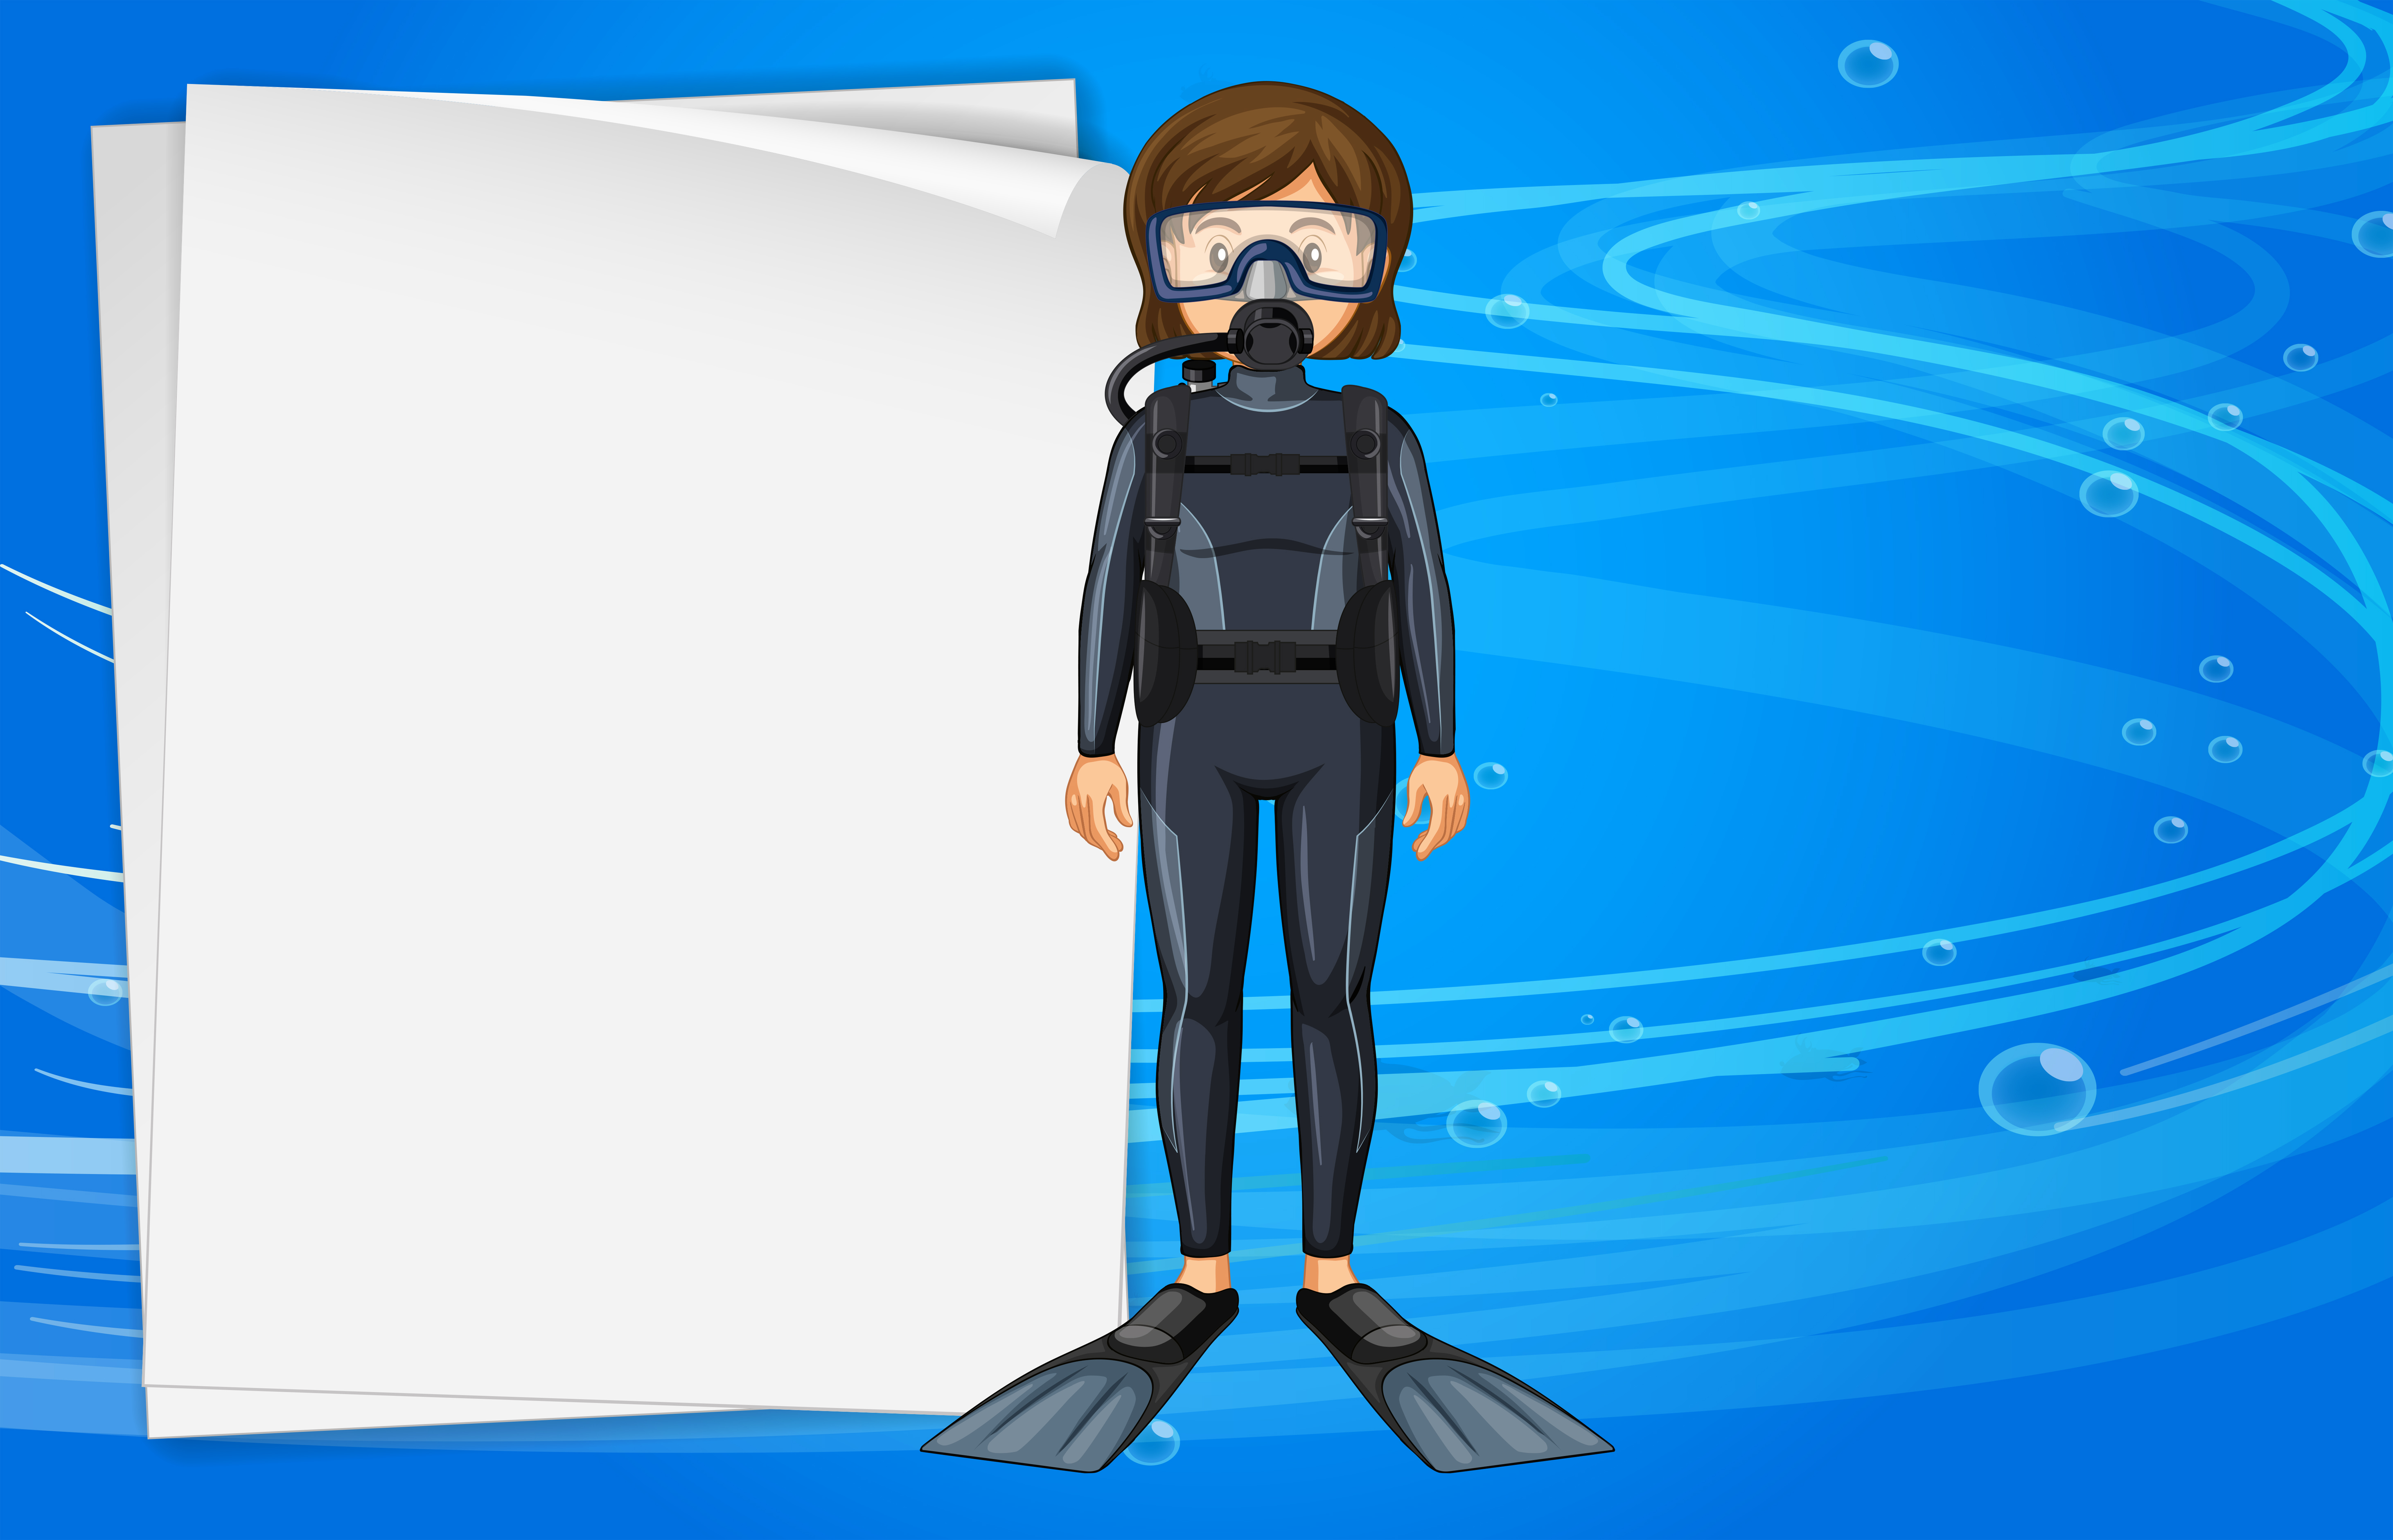
\includegraphics[width=10cm]{plongeuse}};
\node[above right=3pt,font=\scriptsize] at (pic.south west) {image: Freepik.com};
%%%%% zones
\begin{scope}[every path/.style={fill=red,opacity=0.6}]
%%% sinus
\fill[rotate around={20:(0.1,2.4)}] (0.1,2.4) circle (2pt and 1pt);
\fill[rotate around={-20:(0.5,2.4)}] (0.5,2.4) circle (2pt and 1pt);
%%% oreilles
\fill (-0.12,2.1) circle (1pt and 3pt);
\fill (0.7,2.1) circle (1pt and 3pt);
%%% masque
\fill[opacity=0.3,rounded corners=1pt] (-0.05,2) -- ++(0,0.35) -- ++(0.7,-0.01) -- ++(0,-0.32)  -- ++(-0.2,0) -- ++(-0.1,0.2) -- ++(-0.1,0) -- ++(-0.1,-0.2) -- cycle;
%%% dents
\fill (0.31,1.8) circle (3pt and 1pt);
%%% poumons
\fill (0.1,1.25) circle (3pt and 5pt);
\fill (0.5,1.25) circle (3pt and 5pt);
%%% ventre
\fill (0.3,0.6) circle (5pt);
\end{scope}

\def\xx{-2.5}
\def\start{1.3,3.5}
%%% Masque
\uncover<2-4,20>{\draw<2->[stealth-] (\xx,0.44)node[left]{Masque} -- ++(1,0)  -- (0.1,2.1);}
%%% Ventre
\uncover<5-7,20>{\draw<5->[stealth-] (\xx,-2.4)node[left]{Ventre} -- ++(1,0) -- (0.3,0.6);}
%%% Dents
\uncover<8-10,20>{\draw<8->[stealth-] (\xx,-0.54)node[left]{Dents} -- ++(1,0) -- (0.31,1.8);}
%%% Sinus
\uncover<11-13,20>{\draw<11->[stealth-] (\xx,2.40)  -- (0.1,2.4)  node[pos=0,left]{Sinus};}
\uncover<11-13,20>{\draw<11-> (0.5,2.4) -| ++(0,0.2) -- ([xshift=1cm]\xx,2.40) -- (\xx,2.40);}
%%% Oreilles
\uncover<14-16,20>{\draw<14->[stealth-] (\xx,1.42)node[left]{Oreilles} -- ++(1,0) -- (-0.12,2.1);}
\uncover<14-16,20>{\draw<14-> (0.7,2.1) -| ++(0,0.05) -- ++(-1,0) -- ([xshift=1cm]\xx,1.42) -- (\xx,1.42);}
%%% Poumons
\draw<17->[stealth-] (\xx,-1.52)node[left]{Poumons} -- ++(1,0) -- (0.1,1.25);
\draw<17-> (0.5,1.25) -- ([xshift=1cm]\xx,-1.52) -- (\xx,-1.52);

%%% Masque
\node<2-4> (malert) [below right,font=\tiny] at (\start){%
  \begin{minipage}{95pt}
    \begin{alertblock}{Le masque}
      Effet de succion sur les yeux
    \end{alertblock}
  \end{minipage}
};
\node<3-4> (mblock) [right,below,font=\tiny] at (malert.south) {\begin{minipage}{95pt}\begin{block}{Si ça arrive}Pas grave\end{block}\end{minipage}};
\node<4>            [right,below,font=\tiny] at (mblock.south) {\begin{minipage}{95pt}\begin{exampleblock}{Prévention}Souffler dans le masque par le nez à la descente. Ne pas trop serrer le masque.\end{exampleblock}\end{minipage}};
%%% Ventre
\node<5-7> (valert) [below right,font=\tiny] at (\start){%
  \begin{minipage}{95pt}
    \begin{alertblock}{Du gaz dans les intestins}
      Gaz de digestion $\Rightarrow$ douleurs au ventre à la remontée
    \end{alertblock}
  \end{minipage}
};
\node<6-7> (vblock) [right,below,font=\tiny] at (valert.south) {\begin{minipage}{95pt}\begin{block}{Si ça arrive}Ne pas se retenir.\end{block}\end{minipage}};
\node<7>             [right,below,font=\tiny] at (vblock.south) {\begin{minipage}{95pt}\begin{exampleblock}{Prévention}Pas de choucroute la veille~!\end{exampleblock}\end{minipage}};
%%% Dents
\node<8-10> (dalert) [below right,font=\tiny] at (\start){%
  \begin{minipage}{95pt}
    \begin{alertblock}{Des cavités dans les dents}
      Bulle d'air coincée dans une cavité $\Rightarrow$ douleurs à la remontée, peut endommager la dent.
    \end{alertblock}
  \end{minipage}
};
\node<9-10> (dblock) [right,below,font=\tiny] at (dalert.south) {\begin{minipage}{95pt}\begin{block}{Si ça arrive}Faire sortir la bulle, sinon se préparer à une remontée douloureuse.\end{block}\end{minipage}};
\node<10>             [right,below,font=\tiny] at (dblock.south) {\begin{minipage}{95pt}\begin{exampleblock}{Prévention}Aller chez le dentiste tous les ans~!\end{exampleblock}\end{minipage}};
%%% Sinus
\node<11-13> (salert) [below right,font=\tiny] at (\start)  {%
  \begin{minipage}{95pt}
    \begin{alertblock}{Les sinus bouchés}
      Bulles d'air coincées dans les sinus $\Rightarrow$ douleurs à la remontée et à la descente.
    \end{alertblock}
  \end{minipage}
};
\node<12-13> (sblock) [right,below,font=\tiny] at (salert.south) {\begin{minipage}{95pt}\begin{block}{Si ça arrive}Prévenir le GP tout de suite~! Ne pas forcer~! Pas de médicaments~!\end{block}\end{minipage}};
\node<13>            [right,below,font=\tiny] at (sblock.south) {\begin{minipage}{95pt}\begin{exampleblock}{Prévention}On ne plonge pas enrhumé(e)~!\end{exampleblock}\end{minipage}};
%%% oreilles
\node<14-16> (oalert) [below right,font=\tiny] at (\start) {\begin{minipage}{95pt}\begin{alertblock}{Oreilles bouchées}Oreille(s) non équilibrée(s) à la descente/remontée.\end{alertblock}\end{minipage}};
\node<15-16> (oblock) [right,below,font=\tiny] at (oalert.south) {\begin{minipage}{95pt}\begin{block}{Si ça arrive}Prévenir le GP tout de suite~! On ne force pas~!\end{block}\end{minipage}};
\node<16>            [right,below,font=\tiny] at (oblock.south) {\begin{minipage}{95pt}\begin{exampleblock}{Prévention}On ne plonge pas enrhumé(e)~! On équilibre fréquemment \Emph{uniquement} à la descente.\end{exampleblock}\end{minipage}};
%%% Poumons
\node<17-19> (palert) [below right,font=\tiny] at (\start){%
  \begin{minipage}{95pt}
    \begin{alertblock}{Surpression dans les poumons}
      Accident le plus grave~! Arrive lors d'une remontée en apnée ou sous expiration insuffisante.
    \end{alertblock}
  \end{minipage}
};
\node<18-19> (pblock) [right,below,font=\tiny] at (palert.south) {\begin{minipage}{95pt}\begin{block}{Si ça arrive}Mesures d'urgences.\end{block}\end{minipage}};
\node<19>             [right,below,font=\tiny] at (pblock.south) {%
  \begin{minipage}{95pt}
    \begin{exampleblock}{Prévention}
      \begin{itemize}
        \item \emph{Pas d'apnée} en plongée, 
        \item \Emph{jamais} à la remontée.
        \item Souffler \emph{suffisamment} à la remontée,
        \item remonter de façon \emph{contrôlée} et \emph{lente}.
      \end{itemize}
    \end{exampleblock}
  \end{minipage}
};
%%% résumé
\node<20> [below right,font=\tiny,yshift=2pt] at (\start) {%
  \begin{minipage}{95pt}
    \begin{exampleblock}{Au final}
      \begin{itemize}
        \item Souffler dans le masque par le nez à la descente. Ne pas trop serrer le masque.
        \item Pas de choucroute la veille~!
        \item Aller chez le dentiste tous les ans~!
        \item On ne plonge pas enrhumé(e)~!
        \item On équilibre les oreilles fréquemment \Emph{uniquement} à la descente.
        \item \emph{Pas d'apnée} en plongée,
        \item \Emph{jamais} à la remontée.
        \item Souffler \emph{suffisamment} à la remontée, 
        \item remonter de façon \emph{contrôlée} et \emph{lente}.
      \end{itemize}
    \end{exampleblock}
  \end{minipage}
};
\end{tikzpicture}
\end{frame}
